
	\newpage
% =========================================================	
	\section{Frequenzanalyse} \label{chap:Frequenzanalyse}
% =========================================================
	
	\defi{
		\n 
		Trigonometrische Funktionen (aka solche, die Operationen wie $\sin()$ verwenden), besitzen immer eine Amplitude und eine Frequenz. Einige Probleme in der Praxis (wie z.B. Soundwellen) basieren auf Signalen, die man in ihre einzelnen Frequenzen auftrennen möchte. Solche Signale nimmt man als Summen trigonometrischer Funktionen an und lassen sich oft anschaulich durch ihr "Spektrum" darstellen.
	}

	\sbreak
	\bsp{
		\n
		Gegeben sei folgende "Grundfrequenz":
		\begin{align*} 
 			f(x) = \sum_{k=0}^{\infty}c_k \cdot \cos(kx) 
 		\end{align*}
 		Damit lassen sich alle Signale darstellen, die nur aus Kosinus Überlagerungen bestehen. In dem Fall würde ein Signal, welches nur aus der normalen Kosinusfunktion besteht, ausschließlich das Spektrum $k = 1$ aufweisen. Eine gerade Linie als Signal hätte das Spektrum: $k = 0$.
 		\n 
 		Also sind die unterschiedlichen $k$ die unterschiedlichen Frequenzen, $c_k$ beschreibt den Gewichtungskoeffizienten. Bei der Frequenzanalyse ist das äquivalent zu der Amplitude der jeweiligen Frequenz. Also der normale Kosinus hat nur die Frequenz $k=1$ mit einer Amplitude von $c_k = 1$, da der Kosinus zwischen Eins und $-1$ schwingt.
		\n %ewpage
		Im Folgenden ein paar Beispiele von Schwingungen und ihren Frequenzspektren:
		\n
		$\cos(x)$: \\
		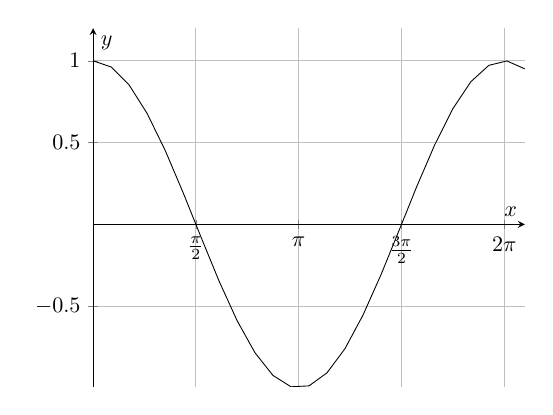
\begin{tikzpicture}[yscale=0.8, xscale=0.8]
					\begin{axis}[ 
						xtick={-3.14159, -1.5708, 0,1.5708,3.14159,4.7123889, 6.28318},
						xticklabels={$-\pi$, $-\frac{\pi}{2}$, $0$,$\frac{\pi}{2}$,$\pi$,$\frac{3\pi}{2}$,$2\pi$},
						axis lines=middle,
						ymax=1.2,
						grid=major,
						xlabel=$x$,
						ylabel=$y$,
						]
						\addplot[domain=0:2.1*pi] {cos(deg(x))} node[left]{};
					\end{axis}
				\end{tikzpicture}%
		\qquad
		\begin{tikzpicture}[yscale=0.8, xscale=0.8]
			\begin{axis}[
				axis lines=middle,
				xlabel=$k$,
				ylabel=$c_k$,
				ymin=0,
				%grid=major,
				ymax=1,
				xtick={0, 1, 2, 3, 4, 5, 6},
				xticklabels={0, 1, 2, 3, 4, 5, 6},
				enlargelimits,
				]
				\addplot[domain=0:6] {0} node[left]{};
				\tikzMegaFatLine{}{1,0}{1,1}
			\end{axis}
		\end{tikzpicture}%
		\newpage
		$0.5 \cdot \cos(x) + 0.5 \cdot \cos(2x)$: \\
%
		\noindent 
		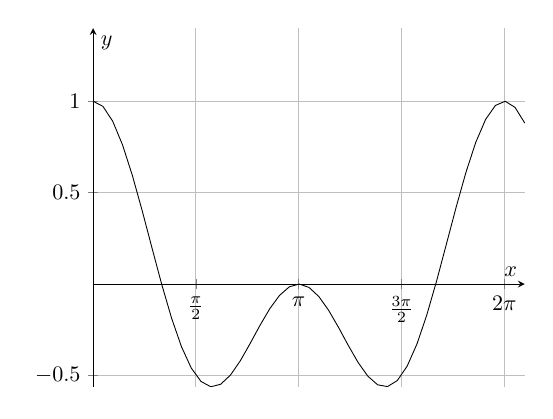
\begin{tikzpicture}[yscale=0.8, xscale=0.8]
			\begin{axis}[ 
				samples=45,
				xtick={-3.14159, -1.5708, 0,1.5708,3.14159,4.7123889, 6.28318},
				xticklabels={$-\pi$, $-\frac{\pi}{2}$, $0$,$\frac{\pi}{2}$,$\pi$,$\frac{3\pi}{2}$,$2\pi$},
				axis lines=middle,
				grid=major,
				ymax=1.4,
				xlabel=$x$,
				ylabel=$y$,
				]
				\addplot[domain=0:2.1*pi] {0.5*cos(deg(x)) + 0.5*cos(2*deg(x))} node[left]{};
			\end{axis}
		\end{tikzpicture}%
		\qquad
		\begin{tikzpicture}[yscale=0.8, xscale=0.8]
			\begin{axis}[
				axis lines=middle,
				xlabel=$k$,
				ylabel=$c_k$,
				ymin=0,
				ymax=1,
				%grid=major,
				xtick={0, 1, 2, 3, 4, 5, 6},
				xticklabels={0, 1, 2, 3, 4, 5, 6},
				enlargelimits,
				]
				\addplot[domain=0:6] {0} node[left]{};
				\tikzMegaFatLine{}{1,0}{1,0.5}
				\tikzMegaFatLine{}{2,0}{2,0.5}
			\end{axis}
		\end{tikzpicture}%
		\n \n
		$0.1 + 0.3 \cdot \cos(2x) + 0.6 \cdot \cos(6x)$: \\
%
		\noindent 
		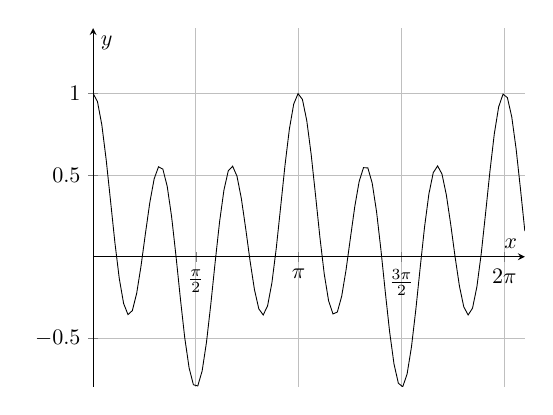
\begin{tikzpicture}[yscale=0.8, xscale=0.8]
			\begin{axis}[ 
				samples=100,
				xtick={-3.14159, -1.5708, 0,1.5708,3.14159,4.7123889, 6.28318},
				xticklabels={$-\pi$, $-\frac{\pi}{2}$, $0$,$\frac{\pi}{2}$,$\pi$,$\frac{3\pi}{2}$,$2\pi$},
				axis lines=middle,
				grid=major,
				ymax=1.4,
				xlabel=$x$,
				ylabel=$y$,
				]
				\addplot[domain=0:2.1*pi] {0.1 + 0.3*cos(2*deg(x)) + 0.6*cos(6*deg(x))} node[left]{};
			\end{axis}
		\end{tikzpicture}%
		\qquad
		\begin{tikzpicture}[yscale=0.8, xscale=0.8]
			\begin{axis}[
				axis lines=middle,
				xlabel=$k$,
				ylabel=$c_k$,
				ymin=0,
				ymax=1,
				%grid=major,
				xtick={0, 1, 2, 3, 4, 5, 6},
				xticklabels={0, 1, 2, 3, 4, 5, 6},
				enlargelimits,
				]
				\addplot[domain=0:6] {0} node[left]{};
				\tikzMegaFatLine{}{0,0}{0,0.1}
				\tikzMegaFatLine{}{2,0}{2,0.3}
				\tikzMegaFatLine{}{6,0}{6,0.6}
			\end{axis}
		\end{tikzpicture}%
	}
	
	\newpage
	\subsection{Diskrete Fourier-Transformation}
	
	\defi{
		\n 
		Die Idee hinter der Fourier-Transformation ist es, ein periodisches, diskretes Signal als Frequenzspektrum auszudrücken.
		Dies wird z.B. häufig im Zusammenhang mit Sound-Effekten ein "Muss".
		\n
		Die Eingabe einer Fourier-Transformation ist ein Vektor $v$, der aus Stützwerten (wie bei Interpolation) besteht. Diese Stützwerte sind immer äquidistant und im Intervall $[0, 2 \pi)$. Warum dieses Intervall? Naja, alle trigonometrischen Funktionen sind $2 \pi$ periodisch. Aus demselben Grund ist auch die obere Intervallgrenze $2\pi$ nicht mehr im Intervall, da es immer derselbe Wert sein muss wie bei $x=0$. Außerdem ähnlich zu Interpolation ist jetzt das Prinzip, das wir anwenden. Im Grunde machen wir einfache Interpolation mithilfe von Basisfunktionen (siehe \refChapter{chap:basisfunktionen}), nur mit trigonometrischen Basisfunktionen im komplexen Bereich, um 3D Signale abdecken zu können.
		\n
		Wenn man es implementiert, erkennt man, dass es sich lediglich um eine Vektor-Matrix Multiplikation handelt, sprich die Laufzeit entspricht $\bigO(n^2)$.
	}

	\sbreak
	\methode{
		\n 
		Die Eingabe für die Diskrete Fourier Transformation (DFT) ist ein Vektor $v$. \\
		Mit 
		\begin{align} 
			\omega = \exp \l(i \cdot \frac{2 \pi}{n} \r) 
 		\end{align}
		und mit $n$ als die Größe des Eingabevektors $v$ ergibt sich die Formel:
		\begin{align} 
 			\DFT(v) := c_k = \frac{1}{n} \cdot \sum_{j=0}^{n-1}v_j \cdot \compl{\omega}^{jk} 
 		\end{align}
		Die Formel für die Inverse Diskrete Fourier Transformation (IDFT):
		\begin{align} 
 			\IDFT(c) := v_j = \sum_{k=0}^{n-1}c_k \cdot \omega^{jk}
		\end{align}
		\n
		In Matrix-Vektor Schreibweise schön darstellbar:
		\begin{align}
			\nvector{
				c_0 \\ c_1 \\ \vdots \\ c_{n-1}
			}
			 = c = M_{\DFT, n} \cdot v = \frac{1}{n}
			\begin{bmatrix}
				1 & 1 & 1 & \dots & 1 \\
				1 & \compl{\omega}^1 & \compl{\omega}^2 & \dots & \compl{\omega}^{(n-1)}\\
				\vdots & \vdots & \vdots & \ddots & \vdots\\
				1 & \compl{\omega}^{n-1} & \compl{\omega}^{2 \cdot (n-1)} & \dots & \compl{\omega}^{(n-1)(n-1)}
			\end{bmatrix} \cdot 
			\nvector{
				v_0 \\ v_1 \\ \vdots \\ v_{n-1}
			}
		\end{align}
		Das Inverse: 
		\begin{align}
			\nvector{
				v_0 \\ v_1 \\ \vdots \\ v_{n-1}
			}
			 = v = M_{\IDFT, n} \cdot c = 
			\begin{bmatrix}
				1 & 1 & 1 & \dots & 1 \\
				1 & \omega^1 & \omega^2 & \dots & \omega^{(n-1)}\\
				\vdots & \vdots & \vdots & \ddots & \vdots\\
				1 & \omega^{n-1} & \omega^{2 \cdot (n-1)} & \dots & \omega^{(n-1)(n-1)}
			\end{bmatrix} \cdot 
			\nvector{
				c_0 \\ c_1 \\ \vdots \\ c_{n-1}
			}
		\end{align}
	}

	\sbreak
	\defi{
		\n 
%		Es gelten folgende Zusammenhänge (die ich nicht beweisen werde, schaut dafür in entsprechende Musterlösungen):
		Außerdem können wir aus unserem Omega (also die Grundfrequenz) noch ein paar Infos ableiten:
		\begin{align*}
			\omega &= \exp \l(i \cdot \frac{2 \pi}{n} \r) \\
				&= \cos \l(\frac{2 \pi}{n} \r) + i \cdot \sin \l(\frac{2 \pi}{n} \r) \\
			\compl{\omega} &= \cos \l(\frac{2 \pi}{n} \r) - i \cdot \sin \l(\frac{2 \pi}{n} \r) = \omega^{-1}
		\end{align*}
		Da es also eigentlich nur einer Kosinus Kurve (im Realteil) und einer Sinuskurve (im Imaginärteil) entspricht, können wir eine Symmetrie und Periodik ableiten:
		\begin{align} 
			\omega^{k \cdot (n -j)} &= \omega^{-kj} &&\text{(Symmetrie)} \\
			w^{k\cdot j} &= w^{k \cdot (n + j)} = w^{(k + n) \cdot j} &&\text{(Periodik)}
		\end{align}
		Daraus können wir uns zum Beispiel für $n=3$ herleiten:
		\begin{align*}
			\compl{\omega}^4 &= \omega^2 = \compl{\omega} \\
			\omega^4 &= \compl{\omega}^2 = \omega
		\end{align*}
	}

	\sbreak
	\bsp{
		\begin{align*} 
 			v = (0, -1, 1)\trans
 		\end{align*}
		\begin{align*}
			\DFT(v) &= \frac{1}{3} \cdot 
			\begin{bmatrix}
				1 & 1 & 1 \\
				1 & \compl{\omega}^1 & \compl{\omega}^2 \\
				1 & \compl{\omega}^2 & \compl{\omega}^4 
			\end{bmatrix} \cdot 
			\nvector{
				0 \\ -1 \\ 1
			} \\
			&= \frac{1}{3} \cdot 
			\nvector{
				0 \\
				-\compl{\omega}^1 + \compl{\omega}^2 \\
				- \compl{\omega}^2 + \compl{\omega}^4
			}
			 = \frac{1}{3} \cdot 
			\nvector{
				0 \\
				\omega - \compl{\omega}\\
				\compl{\omega} - \omega
			}
		\end{align*}
		Jetzt wenden wir die Euler-Formel an (siehe \refChapter{chap:komplexeZahlen}):
		\begin{align*}
			\DFT(v) = \frac{1}{3} \cdot 
			\begin{bmatrix}
				0 \\
				(\cos(\frac{2 \pi}{3}) + i \cdot \sin(\frac{2 \pi}{3})) - (\cos(\frac{2 \pi}{3}) - i \cdot \sin(\frac{2 \pi}{3}))\\
				(\cos(\frac{2 \pi}{3}) - i \cdot \sin(\frac{2 \pi}{3})) - (\cos(\frac{2 \pi}{3}) + i \cdot \sin(\frac{2 \pi}{3}))
			\end{bmatrix}
		\end{align*}
		Mit 
		\begin{align*}
			\cos\l(\frac{2 \pi}{3}\r) = -0.5 \aae \sin\l(\frac{2 \pi}{3}\r) = \frac{\sqrt{3}}{2}
		\end{align*}
		\begin{align*}
			\DFT(v) &= 
			\nvector{
				0 \\
				(-0.5 + i \cdot \frac{\sqrt{3}}{6}) - (-0.5 - i \cdot \frac{\sqrt{3}}{6}) \\
				(-0.5 - i \cdot \frac{\sqrt{3}}{6}) - (-0.5 + i \cdot \frac{\sqrt{3}}{6})
			} \\
			&= 
			\nvector{
				0 \\
				(0 + i \cdot \frac{2\sqrt{3}}{6})\\
				(0 - i \cdot \frac{2\sqrt{3}}{6})
			}
		\end{align*}
	}


	\newpage
	\subsection{Schnelle (Inverse) Fourier-Transformation}
	
	\defi{
		\n 
		Die Fourier-Transformation lässt sich schneller implementieren.
		Die Idee hinter dieser schnellen Variante ist es, mithilfe des sogenannten "Butterfly-Operators" die Menge an redundanten Operationen durch Rekursion zu verkleinern. Dafür sortiert man in der sogenannten "Sortier-Phase" den Eingabevektor nach den Einträgen mit gerade und ungeraden Indizes rekursiv. Danach wendet man oben genannten Operator in der "Kombinationsphase" an und geht dabei die Rekursion Ebenen wieder nach oben.\\
		Es wird sogar deutlich schneller, die neue Laufzeit von IFFT (= Inverse Fast Fourier Transformation) liegt in $\bigO(n \cdot \log(n))$. \\
		Wir nutzen dafür die zwei Eigenschaften von Omega:
		\begin{align*} 
 			\omega^{k \cdot (n -j)} &= \omega^{-kj} &&\text{(Symmetrie)} \\
 			w^{k\cdot j} &= w^{k \cdot (n + j)} = w^{(k + n) \cdot j} &&\text{(Periodik)}
 		\end{align*}
	}

	\sbreak
	\methode{ Butterfly-Operator
		\n 
		Zwei Einträge eines Vektors $a_j$ und $b_j$ mit demselben Index $j$ werden immer zusammen mit dem Butterfly-Operator verbunden. Mit $\BFO$ als Butterfly-Operator ist definiert:
		\begin{align}
			\BFO(a_j, b_j) := (a_j + w^j \cdot b_j, a_j - w^j \cdot b_j)
		\end{align}
		Das Ergebnis sind die Einträge der neuen Vektoren.
		%
	}
		\picC{bfo.png}{0.35}{Der $\BFO$ schöner dargestellt. Links von dem Kreis ist die Eingabe (wobei streng genommen das $w^j$ auch eine Eingabe ist und rechts jeweils die Ausgaben, die jeweils die Vektor-Einträge der Eingabe überschreiben.}

	\newpage
	
	\bsp{\n
		Gegeben seien zwei Arrays mit jeweils einem Eintrag:
		\begin{align*}
			a_0 = 3 \qquad b_0 = 5
		\end{align*}
		Nun wenden wir den Butterfly-Operator an. Wir merken uns, dass unser Index $j = 0$ ist.
		\n
		Unser Ergebnis ist dann ein zweidimensionaler Vektor $z$ mit:
		\begin{align*}
			z &= \nvector{a_0 + w^0 \cdot b_0 \\ a_0 - w^0 \cdot b_0} \\
				&= \nvector{3 + 1 \cdot 5 \\ 3 - 1 \cdot 5} \\
				&= \nvector{8 \\ -2}
		\end{align*}
	}
	
	\picC{fft.jpg}{0.9}{Typische Skizze einer Fast Fourier Transformation mit 8 Einträgen.}
	
	\defi{
		\n 
		Obiges Bild zeigt die Kombinationsphase, in der die einzelnen Buckets mithilfe des $\BFO$ miteinander kombiniert werden. Links unten von jedem Eintrag steht dabei der Index, den der Eintrag in seinem Bucket hat. Das sind nämlich genau die $j$ Werte beim Kombinieren, wie die Einträge neben den $\BFO$ Strichen zeigt (also dieses Kreuz mit dem Kreis entspricht dem $\BFO$).
		\n 
		Dass die Einträge in jedem Schritt anders benannt wurden, spielt nicht wirklich eine Rolle und soll nur zeigen, dass sich die Werte ändern, nicht aber die Positionen. 
		\n
		Wichtig: $\omega$ ist weiterhin $\exp\l(\frac{2\pi i}{n} \r)$, aber $n$ ist bei jedem Kombinationsschritt anders! So ist $n=2$ bei dem ersten Kombinationsschritt, $n=4$ bei dem danach und so weiter\dots
		\n 
		Auf dem Musterlösungsblatt kann man auch ein rasches Codebeispiel für $\FFT$ von der Übungsleitung finden.
 	}
	%
%	An dieser Stelle ein rasches Codebeispiel für FFT (Pseudo-Code):
%	FUNCTION [v[0], ..., v[n-1]] = IFFT(c[0], ..., c[n-1], n)
%		if n == 1:
%			v[0] = c[0];
%		else:
%			m = n / 2;
%			z1 = IFFT(c[0], c[2], ..., c[n-2], n/2);
%			z2 = IFFT(c[1], c[3], ..., c[n-1], n/2);
%			omega = exp(2 * pi * i / n);
%			for j = 0, ..., m-1:
%				v[j] = z1[j] + omega^j * z2[j];
%				v[m+j] = z1[j] - omega^j * z2[j];
%			end
%		end
%		return v;
